\documentclass{article}
\usepackage[utf8]{inputenc}
\usepackage{textcomp}
\usepackage{amsmath}
\usepackage{amssymb} 
\usepackage[margin=1in]{geometry}
\usepackage{mathtools}
\usepackage{graphicx}
\usepackage{epstopdf}
\usepackage{pdfpages}
\usepackage{enumitem}
\graphicspath{ {./figures/} }
% \usepackage{caption}
% \usepackage{multirow}
% \usepackage{mwe}
% \usepackage{subfig}
% \usepackage{caption}
% \usepackage{float}
% \usepackage{cite}
\usepackage[round]{natbib}
%\usepackage[round]{biblatex}
\bibliographystyle{plainnat}


\title{Floquet Theory Basics \& Code Verification}
\author{Bryan Kaiser}
%\date{October 2016}

\begin{document}

\maketitle

Consider the non-autonomous system, 
\begin{equation}
 \frac{\mathrm{d}\mathbf{x}}{\mathrm{dt}}=\mathbf{A}(t)\mathbf{x}(t)
\end{equation}
where the operator $\mathbf{A}(t)$ is periodic:
\begin{equation}
 \mathbf{A}(t+T)=\mathbf{A}(t)
\end{equation}
Note that while $\mathbf{A}$ may be periodic, $\mathbf{x}$ need not be.
If
\begin{equation}
 \mathbf{x}=\begin{bmatrix*}
  u \\
  v
 \end{bmatrix*}
\end{equation}
then the general solution is a superposition of two solutions $\mathbf{x}_1$ and $\mathbf{x}_2$:
\begin{equation}
 \mathbf{x}(t)=c_1\mathbf{x}_1+c_2\mathbf{x}_2
 =c_1\begin{bmatrix*}
  u_1 \\
  v_1
 \end{bmatrix*}+c_2\begin{bmatrix*}
  u_2 \\
  v_2
 \end{bmatrix*}
\end{equation}
and $c_1$ and $c_2$ are arbitrary, time-independent constants.
The fundamental solution matrix is a matrix in which the columns are the solutions
\begin{equation}
 \boldsymbol{\Phi}(t)=\begin{bmatrix*}
 u_1 & u_2 \\
 v_1 & v_2
 \end{bmatrix*}
\end{equation}
The fundamental matrix $\Phi$ to the original system is \textit{not} unique, as there are many ways to 
choose independent solutions and arbitrary constants. 
%Since the solutions are linearly independent, we call them 
%a fundamental set of solutions and $\Phi$ is a fundamental 
%solution matrix. 
Therefore, we can write the general solution as:
\begin{equation}
 \mathbf{x}(t)=\boldsymbol{\Phi}(t)\mathbf{c}=\begin{bmatrix*}
 u_1 & u_2 \\
 v_1 & v_2
 \end{bmatrix*}
  \begin{bmatrix*}
  c_1 \\
  c_2
 \end{bmatrix*}
 \label{eq:gen_soln}
\end{equation}
Since the arbitrary constants $\mathbf{c}$ are independent of time, we 
can define them using (usually known) the initial conditions:
%At some initial time:
\begin{flalign}
 \mathbf{x}(0)
 %=
 % \mathbf{x}_0 \nonumber \\
  &=\boldsymbol{\Phi}(0)\mathbf{c} %\nonumber \\
  %&=\boldsymbol{\Phi}_0\mathbf{c}
 \label{eq:x_IC}
\end{flalign}
% To demonstrate the generality of the decomposition, let $\mathbf{x}(0)=\mathbf{0}$ and 
% $\boldsymbol{\Phi}(0)=\mathbf{I}$:
% \begin{equation}
%  \mathbf{x}(0)=\begin{bmatrix*}
%   0 \\
%   0
%  \end{bmatrix*}=\boldsymbol{\Phi}(0)\mathbf{c}=\begin{bmatrix*}
%  1 & 0 \\
%  0 & 1
%  \end{bmatrix*}
%   \begin{bmatrix*}
%   c_1 \\
%   c_2
%  \end{bmatrix*}
%  =\begin{bmatrix*}
% c_1 \\
%   c_2
%  \end{bmatrix*}
%  \label{eq:x_IC_example}
% \end{equation}
Since the determinant of the initial fundamental solution matrix, $\text{det}[\Phi_0]$, 
is the value at $t_0$ of the Wronskian of the 
independent solutions $\mathbf{x}_1$ and
$\mathbf{x}_2$, it is non-zero because the two solutions are linearly independent.
Therefore a matrix inverse exists and the constants $\mathbf{c}$ can be obtained:
\begin{equation}
 \mathbf{c}=\boldsymbol{\Phi}(0)^{-1}\mathbf{x}(0)
 \label{eq:obtain_c}
\end{equation}
Equation \ref{eq:obtain_c} can be substituted into Equation \ref{eq:gen_soln}
to obtain the forward propogator, which maps $\mathbf{x}_0$ onto $\mathbf{x}(t)$:
\begin{flalign}
 \mathbf{x}(t)&=\boldsymbol{\Phi}(t)\mathbf{c} \nonumber \\
              &=\boldsymbol{\Phi}(t)\boldsymbol{\Phi}(0)^{-1}\mathbf{x}(0)
 \label{eq:forward_propogator}
\end{flalign}
% to the first equation to form columns of .
% To define the fundamental matrix, we need to define it such that it's determinant 
% must be non-zero and it
Note that the fundamental solution 
matrix must also satisfy the equation:
\begin{equation}
 \frac{\mathrm{d}\boldsymbol{\Phi}}{\mathrm{dt}}=\mathbf{A}(t)\boldsymbol{\Phi}(t)
 \label{eq:matrix_equation}
\end{equation}
Since $\boldsymbol{\Phi}(t)$ is a fundamental matrix, then it can be shown that 
%so must be 
$\mathbf{Y}(t)=\boldsymbol{\Phi}(t)\mathbf{C}$ is also a fundamental matrix, so long as
$\mathbf{C}$ is a non-singular constant matrix (note: for $\mathbf{C}$ to be non-singular, 
$\mathbf{x}(0)\neq\mathbf{0}$). We can then 
choose $\mathbf{Y}(t)=\boldsymbol{\Phi}(t+T)$ to obtain:
\begin{equation}
 \boldsymbol{\Phi}(t+T)=\boldsymbol{\Phi}(t)\mathbf{C}
\end{equation}
% This equation is full set of linearly independent solutions 
% depending on the set of linearly independent initial conditions.
% If we integrate over one period:
%If $\Phi_0=\mathbf{I}$ then $\Phi(t)$ is the prinicipal fundamental matrix
%(every floquet 1). 
%where $\mathbf{C}$ is independent of time and non-singular. 
Now, \textit{if 
$\boldsymbol{\Phi}_0=\mathbf{I}$ then $\boldsymbol{\Phi}(T)$ 
is the prinicipal fundamental solution matrix}, denoted by $^*$:
\begin{flalign} 
 \mathbf{C}&=\boldsymbol{\Phi}^*(0)^{-1}\boldsymbol{\Phi}^*(T) \nonumber \\
           &=\mathbf{I}^{-1}\boldsymbol{\Phi}^*(T) \nonumber \\
           &=\boldsymbol{\Phi}^*(T) 
\end{flalign}
$\boldsymbol{\Phi}_0=\mathbf{I}$ can be imposed without a loss of generality because of 
there is no unique choice for $\boldsymbol{\Phi}$ for any given system.
Therefore the initial condition on $\mathbf{x}$ (Equation \ref{eq:x_IC}) is:
\begin{equation}
 \mathbf{x}_0=\mathbf{c}
\end{equation}
and the forward propogator equation (Equation \ref{eq:forward_propogator}) is:
\begin{flalign}
 \mathbf{x}(t)&=\boldsymbol{\Phi}^*(t)\mathbf{x}_0 %\nonumber \\
 %&=\boldsymbol{\Phi}^*(t)\mathbf{c}
\end{flalign}
and therefore
\begin{flalign}
 \mathbf{x}(T)&=\boldsymbol{\Phi}^*(T)\mathbf{x}_0 %\nonumber \\
 %&=\mathbf{C}\mathbf{x}_0 %\nonumber \\
 \label{eq:Cmapping}
\end{flalign}
Eigenanalysis of $\boldsymbol{\Phi}^*(T)$ selects the eigenvectors of $\boldsymbol{\Phi}^*(T)$ as the initial conditions for normal 
modes that are mapped from the initial conditions to the solutions $\mathbf{x}(T)$ by the eigenvalues 
of $\boldsymbol{\Phi}^*(T)$. 
The eigensystem:
% \begin{equation*}
%  \Phi(0)\mathbf{v}_k(0)=\mathbf{I}\mathbf{v}_k(0)=\mu_k\mathbf{I}\mathbf{v}_k(0)
% \end{equation*}
\begin{flalign}
\mathbf{x}(T)_k&= 
 \boldsymbol{\Phi}^*(T)\mathbf{x}_{0,k} \nonumber \\ &=\boldsymbol{\Phi}^*(T)\mathbf{v}_k \nonumber \\ &=\mu_k\mathbf{I}\mathbf{v}_k
 \nonumber \\ &=\mu_k\mathbf{x}_{0,k}
 %\mathbf{C}\mathbf{v}_k=
\end{flalign}
where subscript $k$ denotes each eigenvalue and eigenvector pair. This mapping
is the core of Floquet analysis. $\mu_k$ are the Floquet multipliers and $\mathbf{x}_k$ are 
the Floquet modes.
% can be generalized for all $t$:
% \begin{equation*}
%   \mathbf{x}(t)_k=\Phi(t)\mathbf{v}_k
% \end{equation*}
%  recall
% \begin{equation}
%  \Phi(t+T)=\Phi(t)\mathbf{C}
%  \label{eq:prinicipal_fundamental_matrix}
% \end{equation}
% Then we can say in general %(again taking $t_0=0$)
% \begin{equation*}
%   \mathbf{x}(t)_k=\Phi(t)\mathbf{v}_k
% \end{equation*}
% and from before:
% \begin{equation*}
%  \Phi(t+T)=\Phi(t)\mathbf{C}
% \end{equation*}
% Floquet modes:
% \begin{flalign*}
%  \mathbf{x}(t+T)_k&=\Phi(t+T)\mathbf{v}_k \nonumber \\
%               &=\Phi(t)\mathbf{C}\mathbf{v}_k \nonumber \\
%    &=\Phi(t)\mu_k\mathbf{I}\mathbf{v}_k \nonumber \\
%    &=\mathbf{x}(t)_k\mu_k
% \end{flalign*}
% The eigenvalues of $\mathbf{C}$ are the Floquet multipliers. 
% So, you can take
% \begin{flalign*}
%  \mathbf{x}(T)_k&=\Phi(T)\mathbf{v}_k \nonumber \\
%               &=\mathbf{C}\mathbf{v}_k \nonumber \\
%    &=\mu_k\mathbf{I}\mathbf{v}_k \nonumber \\
%    &=\mu_kc\mathbf{x}(0)_k
% \end{flalign*}
% where
% \begin{equation*}
%  \mathbf{x}(0)_k=\mathbf{I}\mathbf{v}_k
% \end{equation*}
% and $\mathbf{v}_k$ is independent of time.

Integration of Equation \ref{eq:matrix_equation} for the fundamental solution matrix 
over one 
period 
\begin{equation}
 \int_0^T\frac{1}{\boldsymbol{\Phi}^*}\mathrm{d\boldsymbol{\Phi}^*}
 =\log(\boldsymbol{\Phi}^*(t))\Big|_0^T=\log(\boldsymbol{\Phi}^*(T))
 =\int_0^T\mathbf{A}(t)\hspace{0.5mm}\mathrm{dt}
\end{equation}
yields
\begin{equation}
 \boldsymbol{\Phi}^*(T)=\text{exp}\Big[\int_0^T\mathbf{A}(t)\hspace{0.5mm}\mathrm{dt}\Big]
\end{equation}
which is equivalent in the limit of infinitesimal time steps to the ordered product
of infinitesimal propogators:
\begin{equation}
 \boldsymbol{\Phi}^*(T)=\lim_{\Delta{t}\rightarrow0}\prod_{j=1}^N\mathrm{e}^{\mathbf{A}(t_j)\Delta{t}}
 \label{eq:ordered_product}
\end{equation}
where $t_0+(j-1)\Delta{t}<t_j<t_0+j\Delta{t}$ and $T=t_0+N\Delta{t}$. Alternatively,
Equation \ref{eq:matrix_equation} for the fundamental solution matrix can be solved 
using a conventional time stepping scheme, such as a Runge-Kutta method.
% \begin{equation}
%  \int_0^T\mathrm{d\boldsymbol{\Phi}^*}=\boldsymbol{\Phi}^*(T)-\boldsymbol{\Phi}^*(0)=\boldsymbol{\Phi}^*(T)-\mathbf{I}
%  =\int_0^T\mathbf{A}(t)\cdot\boldsymbol{\Phi}^*(0)\hspace{0.5mm}\mathrm{dt}
%  =\int_0^T\mathbf{A}(t)\cdot\mathbf{I}\hspace{0.5mm}\mathrm{dt}%=
% %  \begin{bmatrix*}
% %   -\alpha{T} & \frac{i}{\omega}(\mathrm{e}^{i\omega{T}}-1) \\
% %   0 & -\beta{T}
% %  \end{bmatrix*} %\quad \text{where} \quad \phi(t)=\omega{t}=2\pi{t}/T
% \end{equation}
% therefore
% \begin{equation}
%  \boldsymbol{\Phi}^*(T)=\mathbf{I}+\int_0^T\mathbf{A}(t)\hspace{1mm}\mathrm{dt}
%  \label{eq:PhiT}
% \end{equation}

%\textcolor{red}{this can be equivalently represented as Farrell. ADD BOOKS}

% \newpage
% \section*{An example 2$\times$2 system}
% Let the system of equations be:
% \begin{equation}
%  \frac{\partial{u}}{\partial{t}}=-\alpha u-v\mathrm{e}^{i\omega{t}},
%  \qquad \frac{\partial{v}}{\partial{t}}=-\beta{} v
%  \label{eq:example}
% \end{equation}
% % \begin{equation*}
% %  \mathbf{x}(t)=
% %  \begin{bmatrix*}
% %   -\alpha & -\mathrm{e}^{i\omega{t}} \\
% %   0 & -\beta
% %  \end{bmatrix*} %\quad \text{where} \quad \phi(t)=\omega{t}=2\pi{t}/T
% % \end{equation*}
% therefore
% \begin{equation}
%  \mathbf{A}(t)=
%  \begin{bmatrix*}
%   -\alpha & -\mathrm{e}^{i\omega{t}} \\
%   0 & -\beta
%  \end{bmatrix*} %\quad \text{where} \quad \phi(t)=\omega{t}=2\pi{t}/T
% \end{equation}
% and the solutions are:
% % \begin{equation*}
% %   v(t)=v_0\mathrm{e}^{-\beta{t}}
% % \end{equation*}
% % and
% % \begin{equation*}
% %  u(t)=u_0\mathrm{e}^{-\alpha{t}}+\frac{v_0}{\beta-i\omega-\alpha}\mathrm{e}^{(i\omega-\beta){t}}
% % \end{equation*}
% \begin{equation}
%  \mathbf{x}(t)=
%  \begin{bmatrix*}
%   u_0\mathrm{e}^{-\alpha{t}}+\frac{v_0}{\beta-i\omega-\alpha}\mathrm{e}^{(i\omega-\beta){t}} \\
%   v_0\mathrm{e}^{-\beta{t}}
%  \end{bmatrix*}
%  \label{eq:analytical_soln}
% \end{equation}
% for the initial conditions
% \begin{equation}
%  \mathbf{x}(0)=
%  \begin{bmatrix*}
%   u_0+\frac{v_0}{\beta-i\omega-\alpha} \\
%   v_0
%  \end{bmatrix*}
% \end{equation}
% % Elementwise solutions to Equation \ref{eq:matrix_equation} for the principal solution matrix for 
% % this particular case:
% % % \begin{equation}
% % %  \frac{\partial\Phi_{ij}}{\partial{t}}={A}_{ij}\Phi_{ij}
% % % \end{equation}
% % are
% % \begin{flalign}
% %  \Phi_{ij}^*(t)&=\mathrm{e}^{{A}_{ij}}\Phi_{ij}^*(0) \nonumber \\
% %   &=\mathrm{e}^{{A}_{ij}}I_{ij}(0)
% % \end{flalign}
% % therefore 
% The periodic term in $\mathbf{A}$ integrates to zero, therefore the 
% principal fundamental solution matrix (denoted by $^*$) is
% \begin{equation}
%  \boldsymbol{\Phi}^*(T)
% %  =\begin{bmatrix*}
% %   1-\alpha{T} & \frac{i(\mathrm{e}^{i\omega{T}}-1)}{\omega} \\
% %   0 & 1-\beta{T}
% %  \end{bmatrix*}
%  =\begin{bmatrix*}
%   \mathrm{e}^{-\alpha{T}} & 0 \\
%   0 & \mathrm{e}^{-\beta{T}}
%  \end{bmatrix*}
% \end{equation}
% which has the eigenvalues (Floquet multipliers):
% % \begin{equation*}
% %  (1-\alpha{T}-\lambda)(1-\beta{T}-\lambda)=0
% % \end{equation*}
% \begin{equation}
%  \mu_1=\mathrm{e}^{-\alpha{T}} \qquad \mu_2=\mathrm{e}^{-\beta{T}}
%  \label{eq:multipliers}
% \end{equation}
% and the eigenvectors (initial conditions for the Floquet modes):
% \begin{equation}
%  \mathbf{v}_1=\begin{bmatrix*}
%   1 \\
%   0 
%  \end{bmatrix*}
% \qquad
%  \mathbf{v}_2
% %  =\begin{bmatrix*}
% %   \frac{i(\mathrm{e}^{i\omega T}-1)}{\omega{T}(\alpha-\beta)} \\
% %   1 
% %  \end{bmatrix*}
%  =\begin{bmatrix*}
%   0 \\
%   1 
%  \end{bmatrix*}
%  \label{eq:eigenvecs}
%  \end{equation}
%  The two independent solutions of $\mathbf{x}(T)$ can be use to form another fundamental solution matrix:
% %  \begin{equation}
% %  \mathbf{x}(T)=
% %  \begin{bmatrix*}
% %   u_0\mathrm{e}^{-\alpha{T}}+\frac{v_0}{\beta-i\omega-\alpha}\mathrm{e}^{-\beta{T}} \\
% %   v_0\mathrm{e}^{-\beta{T}}
% %  \end{bmatrix*}
% % \end{equation}
% %  are
% %  \begin{equation}
% %  \mathbf{x}(T)_1=
% %  \begin{bmatrix*}
% %   u_0\mathrm{e}^{-\alpha{T}} \\
% %   0
% %  \end{bmatrix*}
% % \end{equation}
% % \begin{equation}
% %  \mathbf{x}(T)_2=
% %  \begin{bmatrix*}
% %   \frac{v_0}{\beta-i\omega-\alpha}\mathrm{e}^{-\beta{T}} \\
% %   v_0\mathrm{e}^{-\beta{T}}
% %  \end{bmatrix*}
% % \end{equation}
% % such that 
% \begin{equation}
%  \mathbf{x}(T)=\boldsymbol{\Phi}(T)\mathbf{c}=\begin{bmatrix*}
%   \mathrm{e}^{-\alpha{T}} & \frac{\mathrm{e}^{-\beta T}}{\beta-i\omega-\alpha} \\
%   0 & \mathrm{e}^{-\beta{T}}
%  \end{bmatrix*}
%  \begin{bmatrix*}
%   u_0 \\
%   v_0
%  \end{bmatrix*}
%  \label{eq:final_matrix}
% \end{equation}
% Note that this fundamental solution matrix is not the prinicipal fundamental solution matrix because 
% it could not arise from the initial condition $\Phi_0=\mathbf{I}$. Both sets of initial conditions from 
% the eigenvectors of the prinicipal fundamental solution matrix (Equations \ref{eq:eigenvecs}) can be used to map the 
% the solutions from time $t=0$ to time $t=T$, as 
%  in Equation \ref{eq:Cmapping}:
%  \begin{equation}
%   \mathbf{x}(T)_k=\boldsymbol{\Phi}^*(T)\mathbf{v}_k
%  \end{equation}
% Floquet mode $k=1$ %corresponds to selecting $u_0=0,v_0=1$:
%  \begin{equation}
%   %\mathbf{x}(T)_k&=\boldsymbol{\Phi}^*(T)\mathbf{v}_k \nonumber \\
%   \mathbf{x}(T)_1=\boldsymbol{\Phi}^*(T)\mathbf{v}_1=\begin{bmatrix*}
%   \mathrm{e}^{-\alpha{T}} & 0 \\
%   0 & \mathrm{e}^{-\beta{T}}
%  \end{bmatrix*}
%  \begin{bmatrix*}
%   1 \\
%   0 
%  \end{bmatrix*}
%  =\mu_1\mathbf{v}_1
%  \end{equation}
%  corresponds to selecting:
%  \begin{equation}
%   u_0=0,\qquad v_0=1
%  \end{equation}
%  in Equation \ref{eq:analytical_soln}.% at time $t=T$.
% Floquet mode $k=2$
%  \begin{equation}
%   %\mathbf{x}(T)_k&=\boldsymbol{\Phi}^*(T)\mathbf{v}_k \nonumber \\
%   \mathbf{x}(T)_2=\boldsymbol{\Phi}^*(T)\mathbf{v}_2=\begin{bmatrix*}
%   \mathrm{e}^{-\alpha{T}} & 0 \\
%   0 & \mathrm{e}^{-\beta{T}}
%  \end{bmatrix*}
%  \begin{bmatrix*}
%   0 \\
%   1 
%  \end{bmatrix*}
%  =\mu_2\mathbf{v}_2
%  \end{equation}
% corresponds to selecting
% \begin{equation}
%  u_0=-\Big(\frac{\mathrm{e}^{-\beta{T}}}{\beta-i\omega-\alpha}+\mathrm{e}^{-\alpha{T}}\Big), \qquad v_0=1
% \end{equation}
% in Equation \ref{eq:analytical_soln}.% at time $t=T$.
% The Floquet exponents are defined as 
% \begin{equation*}
%  \mu_k=\mathrm{e}^{\gamma_k{T}}
% \end{equation*}
% which indicate Floquet mode frequencies exist for imaginary $\gamma_k$ and 
% that if the real part of $\gamma_k$ is greater than unity growth will occur.
%  \begin{equation*}
%   \begin{bmatrix*}
%   u_0\mathrm{e}^{-\alpha{T}}+\frac{v_0}{\beta-i\omega-\alpha}\mathrm{e}^{-\beta{T}} \\
%   v_0\mathrm{e}^{-\beta{T}}
%  \end{bmatrix*}
%  =\begin{bmatrix*}
%   \mathrm{e}^{-\alpha{T}} & 0 \\
%   0 & \mathrm{e}^{-\beta{T}}
%  \end{bmatrix*}
%  \begin{bmatrix*}
%   1 \\
%   0 
%  \end{bmatrix*}
%  \end{equation*}


% \newpage
% \section*{Verification of the time stepping algorithms}
% \begin{figure}[h!]
% \centering
% 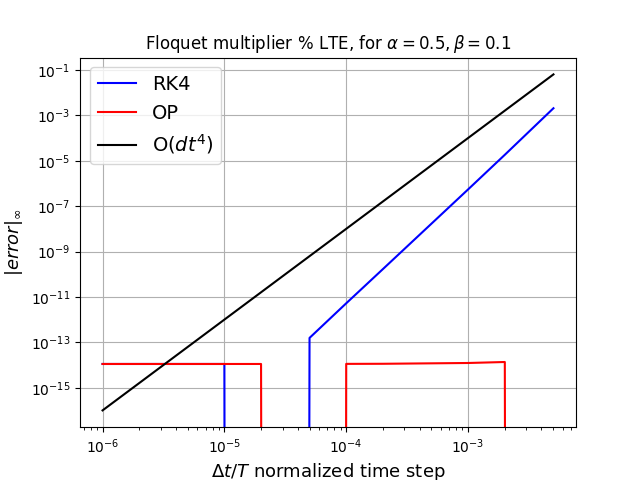
\includegraphics[width=4.1in]{LTE_loglog.png}
% \caption{$L_\infty$ norm of the local (i.e. one time step) Floquet multiplier percent error 
% ($\max[|\lambda_{k,\text{computed}}-\lambda_{k,\text{analytical}}|/|-\lambda_{k,\text{analytical}}|]$) 
% due to temporal truncation
% for the system of equations 
% in Equation \ref{eq:example} as a function of time step divided by period. 
% The principal fundamental solution matrix $\boldsymbol{\Phi}^*(t)$
% was advanced in time explicitly using a 4th order Runge Kutta method (the 
% \textcolor{blue}{blue} line) one time step $\Delta{t}$ 
% and then the 
% percent error was computed between the
% eigenvalues 
% (i.e. Floquet multipliers) of 
% the computed matrix $\boldsymbol{\Phi}^*(t)$ and the exact analytical solutions (Equation \ref{eq:multipliers}). Machine precision is acheived at time step 
% size corresponding to about $3\cdot10^4$ time steps per period. The \textcolor{red}{red} line error was 
% computed by advancing in time using the ordered product in Equation \ref{eq:ordered_product}. A percent error 
% of $\mathcal{O}(10^{-13})$ is approximately machine precision.}
% \end{figure}
% \begin{figure}[h!]
% \centering
% 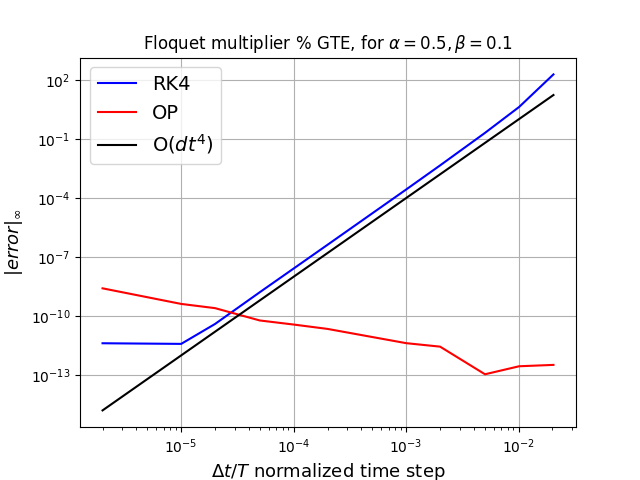
\includegraphics[width=4.1in]{GTE_loglog.png}
% \caption{$L_\infty$ norm of the global (i.e. integrated one period) Floquet multiplier percent error 
% due to temporal truncation
% %($\max[|\lambda_{k,\text{computed}}-\lambda_{k,\text{analytical}}|/|-\lambda_{k,\text{analytical}}|]$) 
% for the system of equations 
% in Equation \ref{eq:example} as a function of time step divided by period. 
% % The principal fundamental solution matrix $\boldsymbol{\Phi}^*(t)$
% % was advanced in time explicitly using a 4th order Runge Kutta method (for which the local truncation error is $\mathcal{O}(\Delta{t}^4)$) one time step $\Delta{t}$ 
% % and then the 
% % percent error was computed between the
% % eigenvalues 
% % (i.e. Floquet multipliers) of 
% % the computed matrix $\boldsymbol{\Phi}^*(t)$ and the exact analytical solutions (Equation \ref{eq:multipliers}). Machine precision is acheived at time step 
% % size corresponding to about $3\cdot10^4$ time steps per period.
% }
% \end{figure}


\newpage
\section*{Mathieu equation example}
Hill's equation are the form:
\begin{equation*}
 \frac{\partial^2y}{\partial{t^2}}+f(t)y=0, 
\end{equation*}
which can be expressed in matrix form as:
 \begin{equation*}
  \begin{bmatrix*}
  y_t \\
  y_{tt}
 \end{bmatrix*}
 =\begin{bmatrix*}
  0 & 1 \\
  -f(t) & 0
 \end{bmatrix*}
 \begin{bmatrix*}
  y \\
  y_t 
 \end{bmatrix*}
 \end{equation*}
 where $y_t$ and $y_{tt}$ are the first and second temporal derivatives of $y$.
Mathieu's equation is a special case of a Hill equation in which the function $f(t)$ takes the form: 
\begin{equation*}
 f(t)=\delta+\varepsilon\cos(t)
\end{equation*}
Hill equations possess the property:
\begin{equation*}
 \det[\Phi^*(T)]=1
\end{equation*}
Which means that the eigenvalues (Floquet multipliers) of $\Phi^*(T)$ 
can be obtained through the relationship:
\begin{equation}
 \mu_{1,2}=\frac{\text{tr}[\Phi^*(T)]\pm\sqrt{\text{tr}[(\Phi^*(T))^2]-4}}{2}
 \label{eq:eigroots}
\end{equation}
So for Hill equations the stability can be determined either by the Floquet multipliers 
or the trace of the monodromy matrix ($\text{tr}[(\Phi^*(T))^2]$). 
The stability of the system in terms of Floquet multipliers is:
\begin{enumerate}[label=(\alph*)]
\item If $|\mu|<1$ (where $|\mu|$ is the complex modulus of $\mu$) then the real part of the corresponding
 Floquet exponent is negative ($\text{Real}[\gamma]<0$) and the Floquet mode is 
 damped. If all of the multipliers $\mu_k$ satisfy this property then the system is 
 \textbf{stable} and decays as $t\rightarrow\infty$.
\item If $|\mu|=1$ then the corresponding
 Floquet exponent is zero ($\text{Real}[\gamma]=0$) and the mode is 
 periodic, although not necessarily oscillating with the base period. 
 If $\mu\pm1+0i$ the mode is periodic with exactly the base period.
 If all modes in the system satisfy this property then the system 
 is \textbf{purely periodic} for all time.
\item If $|\mu|>1$ then the real part of the corresponding
 Floquet exponent is positive ($\text{Real}[\gamma]>0$) and the mode 
 will grow in amplitude as $t\rightarrow\infty$. If any mode satisfies this 
 property, then the system is \textbf{unstable} and grows as $t\rightarrow\infty$.
\end{enumerate}
Equivalently, the stability conditions in terms of the 
trace of the monodromy matrix for Hill equations are:
\begin{enumerate}[label=(\alph*)]
\item For $|\text{tr}[\Phi^*(T)]|<2$ Equation \ref{eq:eigroots} has a pair of complex conjugate 
roots. Since the product 
of the roots is unity, they both must lie in the unit circle. 
Therefore the system is \textbf{stable}.
\item For $|\text{tr}[\Phi^*(T)]|=2$ the roots of Equation \ref{eq:eigroots} are $\mu=1,1$ and
$\mu=-1,-1$. For $\mu=1,1$ the system is \textbf{purely periodic} 
with period $T$. Plug $\mu=-1,-1$ in Equation \ref{eq:eigroots} and the system is \textbf{purely periodic} 
with period $2T$.
\item For $|\text{tr}[\Phi^*(T)]|>2$ Equation \ref{eq:eigroots} has real roots. The product 
of the roots is unity, but one of the complex moduli of the Floquet multipliers is 
less than unity and the other must be greater
than unity, so this case the system is \textbf{unstable}.
\end{enumerate}
Here we verify the estimate of system stability obtained from the Floquet multipliers 
with the stability obtained from the trace of the monodromy matrix for the Mathieu equation.


\newpage
\section*{Code verification of stability calculations}
\begin{figure}[h!]
\centering
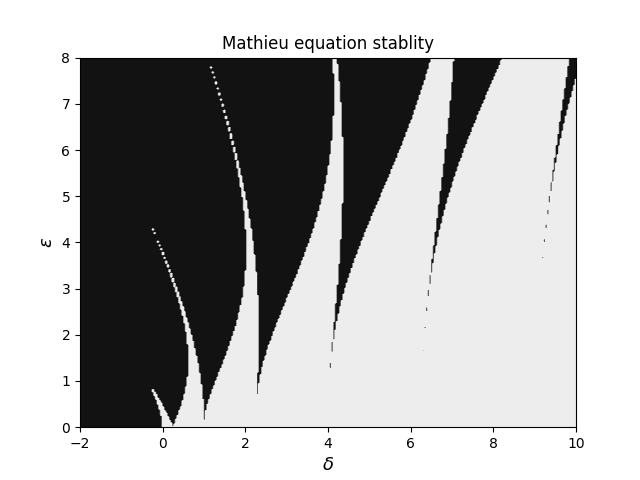
\includegraphics[width=4.5in]{strutt_eig_rk4.png}
\caption{Computed results: a Strutt diagram for the stability of Mathieu's equation (black is unstable, white is 
stable) using the Floquet multiplier method. The results are consistent with analytical 
and numerical solutions in the literature regarding Mathieu's equation (\citet{Kovacic18}).
}
\end{figure}
\begin{figure}[h!]
\centering
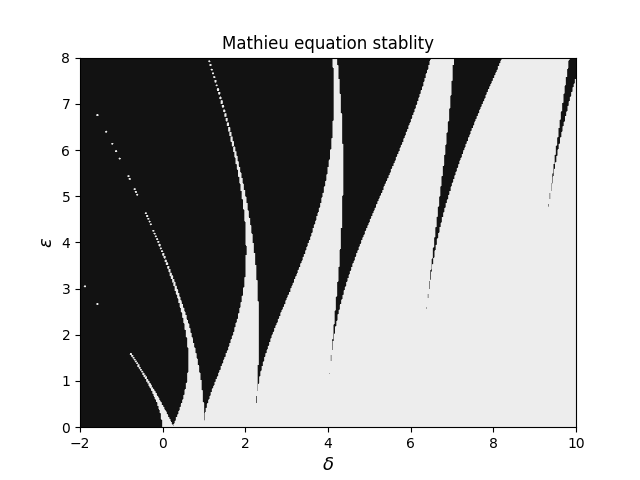
\includegraphics[width=4.5in]{strutt_Tr_rk4.png}
\caption{Computed results: a Strutt diagram for the stability of Mathieu's equation (black is unstable, white is 
stable) using the trace of the monodromy matrix method for Hill equations.
}
\end{figure}

\begin{figure}[h!]
\centering
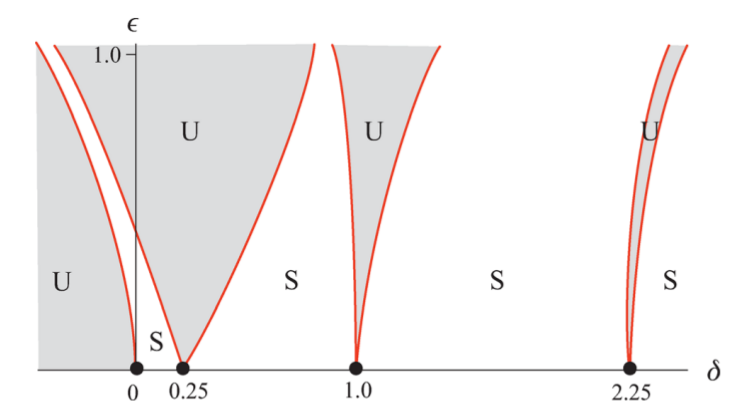
\includegraphics[width=4.5in]{fig3_Kovacic_2018.png}
\caption{A Strutt diagram for the stability of Mathieu's equation from \citet{Kovacic18}.
}
\end{figure}

\newpage
\bibliography{references} 

\end{document}
